\chapter{Functions}

\begin{defn}[function]
    \index{function}
    A \definition{function}{function} $f$
    from a set $D$ to a set $R$
    is an assignment of exactly one element
    $f(x) \in R$ to each element $x \in D$.
    If $f$ is a function from $D$ to $R$, we write
    \begin{equation}
        f:D \to R,
        \label{eq:function_definition}
    \end{equation}
    and say that $f$ \emph{maps} $D$ to $R$.
    A function has four properties:
    \begin{enumerate}
        \item A \definitionintro{domain} $D$ and a \emph{codomain} $R$, both sets,
        \item $\forall x \in D\, \exists\, f(x) \in R$
          which we call the
          \emph{value} of the function \emph{at} $x$,
        \item $D$, $R$, and each value $f(x)$ for each element $x$ are
              determined completely by $f$,
        \item The data constituting $D$, $R$, and the value 
              $f(x) \forall x \in D$
              completely determine $f$.
    \end{enumerate}
\begin{figure}
  \centering
  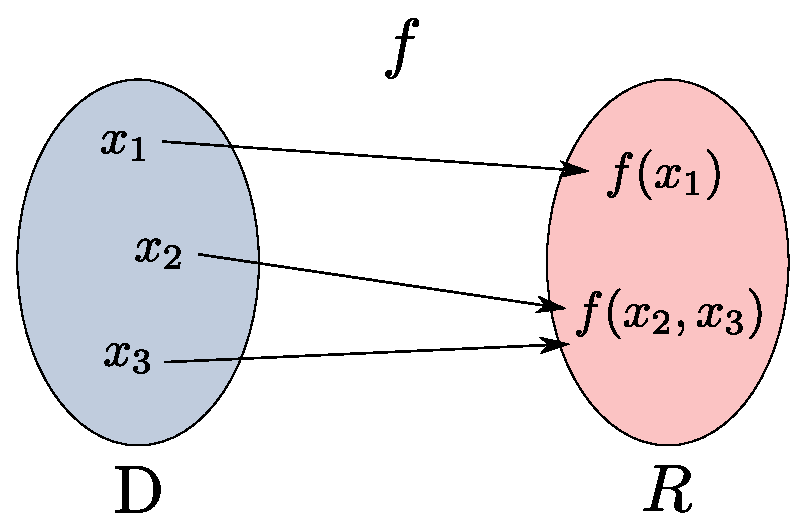
\includegraphics[width=0.4\textwidth]{continuous/functions/function.eps}
  \caption{A function $f$ mapping from $D$ to $R$.
    Note how multiple $x$ values share the same $f(x)$ value.}
  \label{fig:function}
\end{figure}

\end{defn}

One technique that can help us understand functions is by describing them with words,
including mathematical language.
We can discuss the behavior of a function in general,
describing its properties, or we can discuss its behavior in more specific terms,
like when we evaluate a function at a certain value.

We can also talk about functions using visual language,
by way of plots,
arrow diagrams (\figref{fig:function}),
and tables.
% There are, of course, many ways to visually represent a function, but for our purposes these will prove the most useful.
% This includes some numerical displays of functions, like with a table of values.
% We can consider tables to be a visual description of a function because they combines visual formatting with descriptive data to produce a figural representation of a function's properties.

%We will find graphs, in conjunction with the respective mathematical language, 
%to be the most cohesive way to represent functions.
%We should therefore attempt to be able to graph our functions whenever we wish to achieve the best possible understanding of them.

We will combine these techniques in an effort to paint a complete picture of its 
behavior.

\section{Properties of Functions}

Here, we will discuss a number of the properties that will be of interest when we
are describing functions.
Not all of these properties will exist for every type of function.
For example, not all functions will have an inverse 
(described in \secref{sec:inverse}), 
but the nonexistence of an inverse then becomes an important property of the 
function. % WHEN????? Tell the reader where this is useful.

\subsection{Domain and Range}

\begin{defn}[domain]
  The set $D$ of all possible input values on which a function $f$ is defined
  is called the \definition{domain}{domain} of $f$.
\end{defn}

\begin{defn}[range]
  Given a function $f$ defined on a domain $D$,
  the set of all values of $f(x)$
  as $x$ varies throughout $D$ is called
  the \definition{range}{range} or
  \altdefinition{codomain}{codomain} $R$ of $f$.
\end{defn}

In certain areas of mathematics, including calculus,
it is common to define functions without supplying an explicit domain.
Instead, we will implicitly use the
\definitionintro{natural domain}
in these cases.

\begin{defn}[natural domain]
  For a function $f: D \rightarrow R$,
  where $f(x)$ is the value of $f$ at $x$,
  the \definition{natural domain}{natural domain}
  is the set of all values
  \begin{equation}
    \setbuilder{x}{f(x) \in \realnumbers \land  x \in D \cap \realnumbers}.
    \label{eq:functions:naturaldomain}
  \end{equation}
\end{defn}

\begin{defn}[real-valued]
  A function is said to be \definition{real-valued}{real-valued} when
  its domain is exactly equal to the set of $\realnumbers$ of real numbers.
\end{defn}

That is, the domain is equal to to the set of real numbers.
This means that we can put an arbitrary real number into the function and it 
will return a real $y$-value.

The \definition{vertical line test}{vertical line test}
for a function is based on the idea that if
$a$ is in the domain of the function $f$ then the vertical line $x=a$ will 
intersect the graph of $f$ at a single point $ \big(a,f(a)\big)$.
\index{vertical line test}

\begin{figure}
  \begin{center}
    \subfigure[This passes the vertical line test]{\
    \begin{tikzpicture}
      \begin{axis}[
        axis lines = left,
        xlabel = $x$,
        ylabel = {$f(x)$},
        axis y line = center,
        axis x line = middle,
      ]
      \addplot[domain=-5:5, samples=100,]{x^2};
      \addplot[color=blue,thick,dashed] coordinates {(3,0) (3,25) };
      \end{axis}
    \end{tikzpicture}
    }
    \subfigure[This fails the vertical line test]{\
    \begin{tikzpicture}
      \begin{axis}[
        axis lines = left,
        xlabel = $x$,
        ylabel = {$f(x)$},
        axis y line = center,
        axis x line = middle,
      ]
      \addplot[domain=-5:5, samples=100,]{sqrt(x)};
      \addplot[domain=-5:5, samples=100,]{-sqrt(x)};
      \addplot[color=blue,thick,dashed] coordinates {(3,-3) (3,3) };
      \end{axis}
    \end{tikzpicture}
    }
  \end{center}
  \caption{Examples of the vertical line test.}
\end{figure}


\subsection{Dependent and Independent Variables}
  The letter $x$ in the notation $y=f(x)$ is called the 
  \textbf{independent variable} of the function, representing the input value 
  of $f$.
  \index{independent variable}

  The letter $y$ in the notation $y=f(x)$ is called the 
  \textbf{dependent variable}.
  It varies with respect to change in the dependent variable of the function.
  \index{dependent variable}

\subsection{Even and Odd Functions}

For a function $f$ in the form $y=f(x)$, we describe its type of symmetry by 
calling the function \textbf{even}\index{even functions} or 
\textbf{odd}\index{odd functions}.

\begin{defn}[even function]
  An \definition{even function}{even function} $f$
  is one where the property $f(-x)=f(x)$ holds for all values in the domain.
\end{defn}

\begin{ex}
  An example of an even function is the function $f$,
  where $f(x)=x^2$.
  A plot of this function is shown in \figref{fig:functions:even}.

  \begin{figure}
    \begin{center}
    \begin{tikzpicture}
      \begin{axis}[
        axis lines = left,
        xlabel = $x$,
        ylabel = {$x^2$},
        axis y line = center,
        axis x line = middle,
      ]
        \addplot[domain=-5:5, samples=100,]{x^2};
      \end{axis}
    \end{tikzpicture}
    \end{center}
    \caption{$f(x) = x^2$ is an even function.}
    \label{fig:functions:even}
  \end{figure}
\end{ex}

\begin{defn}[odd function]
  An \definition{odd function}{odd function} $f$
  is one where the property $f(-x)=-f(x)$ holds for all values in its domain.
\end{defn}

\begin{ex}
  An example of an odd function is $f(x)=x^3$.
  A plot of this function is shown in \figref{fig:functions:odd}.
  \begin{figure}[H]
    \begin{center}
      \begin{tikzpicture}
        \begin{axis}[
          axis lines = left,
          xlabel = $x$,
          ylabel = {$x^3$},
          axis y line = center,
          axis x line = middle,
        ]
          \addplot[domain=-5:5, samples=100,]{x^3};
        \end{axis}
      \end{tikzpicture}
    \end{center}
    \caption{$f(x)=x^3$ is an odd function.}
    \label{fig:functions:odd}
  \end{figure}
\end{ex}

\subsection{Surjective, Injective, and Bijective Functions}

\begin{defn}[injective]
  If each $f(x)$ value produced by a function $f$ can only be obtained by one 
  unique $x$ value, then we say $f$ is \definition{injective}{injective}, or 
  \altdefinition{one-to-one}{one-to-one}.

  $ f: D \to R $ is injective or one-to-one iff
  \[
    \forall{(x_1 \wedge x_2 \in D)}
    \big[f(x_1)=f(x_2)
    \to x_1=x_2\big].
  \]
  \begin{remark}
    This also means that for injective functions,
    $ x_1 \neq x_2 \to f(x_1) \neq f(x_2)$.
  \end{remark}
\end{defn}

\begin{figure}
    \begin{center}
        \subfigure[The function $f(x)=x^2$ is not \emph{one-to-one} because
        there are two possible $x$-values that can produce each given
        $y$-value.]
        {\
          \begin{tikzpicture}
            \begin{axis}[
              axis lines = left,
              xlabel = $x$,
              ylabel = {$x^2$},
              axis y line = center,
              axis x line = middle,
            ]
              \addplot[domain=-5:5, samples=100,]{x^2};
            \end{axis}
          \end{tikzpicture}
        }
        \hspace{0.2in}%
        \subfigure[The function $f(x)=x^3$ is \emph{one-to-one} because every 
        given $y$-value is mapped from a unique $x$-value.]
        {\
          \begin{tikzpicture}
            \begin{axis}[
              axis lines = left,
              xlabel = $x$,
              ylabel = {$x^3$},
              axis y line = center,
              axis x line = middle,
            ]
              \addplot[domain=-5:5, samples=100,]{x^3};
            \end{axis}
          \end{tikzpicture}
        }
    \end{center}
  \end{figure}
  A function $y=f(x)$ is one-to-one iff its graph intersects each horizontal 
  line at most once.\index{horizontal line test}
\begin{defn}
  \index{onto}
  \index{surjective}
  $f: D \to R $ is \textbf{surjective} or \textbf{onto} iff
    \[\forall (y \in R) \exists  (x \in D) \big[f(x)=y\big]. \]
\end{defn}
\begin{figure}[H]
    \begin{center}
        \subfigure[The function $f(x)=x^2$ is not \emph{surjective} because 
        the values $(-\infty, 0)$ are never reached in its range.]
        {\
          \begin{tikzpicture}
            \begin{axis}[
                ylabel={$f(x)=x^2$},
                axis x line=bottom,
                axis y line=center,
                tick align=outside,
                yticklabels={,,}
                xticklabels={,,}
                xtickmax=10,
              ]
              \addplot[smooth,red]{x^2};
            \end{axis}
          \end{tikzpicture}
        }
        \hspace{0.2in}%
        \subfigure[The function $f(x)=x^3$ is \emph{one-to-one} because all $y$ values from $-\infty, \infty)$ have corresponding $x$-values.]
        {\
          \begin{tikzpicture}
            \begin{axis}[
                ylabel={$f(x)=x^3$},
                axis x line=bottom,
                axis y line=center,
                tick align=outside,
                yticklabels={,,}
                xticklabels={,,}
                xtickmax=10,
              ]
              \addplot[smooth,blue]{x^3};
            \end{axis}
          \end{tikzpicture}
        }
    \end{center}
  \end{figure}

  \begin{defn}
    \index{bijective}
    A function $f:A \to B$ is \textbf{bijective} iff it is \emph{both injective and surjective}.
  \end{defn}
\begin{figure}[H]
    \begin{center}
        \subfigure[The function $f(x)=x^2$ is not bijective.]
        {\
          \begin{tikzpicture}
            \begin{axis}[
                ylabel={$f(x)=x^2$},
                xlabel={$x$},
                axis x line=bottom,
                axis y line=center,
                tick align=outside,
                yticklabels={,,}
                xticklabels={,,}
                xtickmax=10,
              ]
              \addplot[smooth,red]{x^2};
            \end{axis}
          \end{tikzpicture}
        }
        \hspace{0.2in}%
        \subfigure[The function $f(x)=x^3$ is bijective.]
        {\
          \begin{tikzpicture}
            \begin{axis}[
                ylabel={$f(x)=x^3$},
                xlabel={$x$},
                axis x line=bottom,
                axis y line=center,
                tick align=outside,
                yticklabels={,,}
                xticklabels={,,}
                xtickmax=10,
              ]
              \addplot[smooth,blue]{x^3};
            \end{axis}
          \end{tikzpicture}
        }
    \end{center}
  \end{figure}


\subsection{Graphs} \index{graphs}

\begin{defn}
  \index{graph}
    If $f$ is a function with a domain $D$, then its \textbf{graph} is the set
    \[ \Big\{ \big( x,f(x) \big) \Big | x \in D \Big\},\]
    that is, it is the set of all points $(x, f(x))$ where $x$ is in the domain of the function.%
\footnote{Here, the difference between the words \emph{graph} and \emph{plot} is sometimes confusing. Technically speaking, a \emph{graph} is the set defined explicitly here, while a function's \emph{plot} refers to any pictorial representation of a data set. However, since the usage is inconsistent in this text, these formal definitions will usually not apply. It can be safely assumed that as long as we are within the realm of real numbers, all uses of either \emph{graph} or \emph{plot} hereafter simply refer to the pictorial representation of a function's graph in the form of a curve on the cartesian plane.}
\end{defn}

If $ (x,y) $ is a point on $f$, then $y=f(x)$ is the height of the graph above point $x$.
This height might be positive or negative, depending on the sign of $f(x)$.
We use this height relationship to plot functions.
\begin{figure}[H]
    \begin{center}
        \begin{tikzpicture}
          \begin{axis}[
              ylabel={$f(x)$},
              xlabel={$x$},
              axis x line=bottom,
              axis y line=center,
              tick align=outside,
              yticklabels={,,}
              xticklabels={,,}
              xtickmax=10,
            ]
            \addplot[smooth,red]{x+2};
          \end{axis}
        \end{tikzpicture}
      \caption{A plot of the function $f(x)=x+2$}
    \end{center}
  \end{figure}

\section{Composition of Functions}
\label{sec:compositefunctions}
\begin{defn}
  If $f$ and $g$ are functions, then the \textbf{composite} function 
  $f \circ g$, ``$f$ composed with $g$'', is defined by
  \[ (f \circ g)(x)=f\bigl(g(x)\bigr) \text{.} \]
  \begin{remark}
    The domain of $ f \circ g $ consists of the numbers $x$ in the domain of 
    $g$ for which $g(x)$ lies in the domain of $f$.
    See figure~\ref{fig:p1sin1x} for an example of a function which produces 
    indefinite $y$-values for real $x$-values around $x=0$.
  \end{remark}
  \index{composition}
\end{defn}
\begin{ex}
  If
  $f(x)=x^2$
  and
  $g(x)=1-\sqrt{x}$,
  find $ (f \circ g)(x) $ and $ (g \circ f)(x)$.
  \begin{sol}
      We know that $(f \circ g)(x)$ is just $f(g(x))$ so
      \[ f(g(x)) = (1 - \sqrt x )^2. \] For $(g \circ f)(x)$ it is the opposite
      and \[ g(f(x)) = 1 - \sqrt{x^2} ,\]
      which is equivalent to saying \[ g(f(x)) = 1 - \abs{x}. \]
  \end{sol}
\end{ex}

\section{Inverse Functions}\index{inverse functions}\label{sec:inverse}
An inverse function undoes, or inverts, the effects of an original function.
% Old gibberish from when this was in the transcendental section.
%While inverse functions are not, by definition, transcendental, we will look 
%at them in this chapter because they are useful for producing inverse 
%trigonometric functions--functions that are transcendental.
They are useful for producing inverse trigonometric functions--functions that 
are transcendental.

\begin{defn}
  Suppose that $f$ is a one-to-one function on a domain $D$ with range $R$. The 
  \textbf{inverse function} $f^{-1}$ is defined by
  \[ f^{-1}(b)=a \text{ if } f(a)=b. \]
  The domain of $f^{-1}$ is $R$ and the range of $f^{-1}$ is $D$.
  \index{inverse functions}
\end{defn}
In order for an inverse function $f^{-1}(x)$ to exist for a function $f(x)$, 
the original function $f(x)$ must be one-to-one. Otherwise, the resulting 
``inverse function'' would not be a function: more than one output would be 
produced from only one input, and it would not pass the vertical line test.
\begin{figure}[H]
  \begin{center}
    \subfigure[A plot of $f(x)=\sqrt x$.]{\
      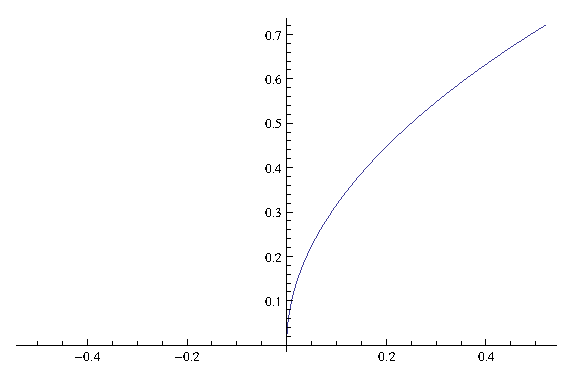
\includegraphics[width=0.3\textwidth]{continuous/functions/sqrtx}
    }
    \subfigure[A plot of $f^{-1}(\sqrt x)=x^2$.]{\
      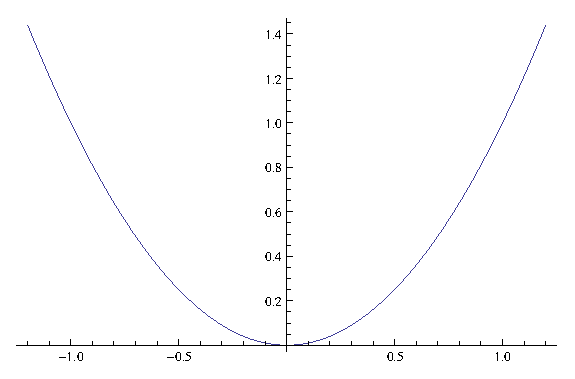
\includegraphics[width=0.3\textwidth]{continuous/functions/x2inv}
    }
  \end{center}
  \label{fig:inversef}
\end{figure}
\begin{remark} \index{composition}\index{inverse functions}
  By definition, either composite of a function and its inverse will return the 
  identity function, where $y=x$. For example:
  \[ (f \circ f^{-1})(x)=f(f^{-1}(x))=x, \]
  or
  \[ (f^{-1} \circ f)(x)=f^{-1}(f(x))=x. \]
\end{remark}

\subsection{Finding Inverse Functions}

To find the inverse of a function $f(x)$, replace $f(x)$ with $y$ and solve for 
$x$ in terms of $y$. Then, interchange $x$ and $y$.
\begin{ex}
  \label{ex:inverses}
  Find the inverse of $y=\frac{1}{2}x+1$, expressed as a function of $x$.
  \begin{sol}
    First, we solve the function for $x$ in terms of $y$.
    \begin{align*}
      y &= \frac{1}{2}x+1 \\
      \intertext{Multiply both sides by $2$.}
      2y &= x + 2 \\
      \intertext{Now subtract $2$ from both sides, and swap the left and right 
          sides of the equation.}
      x &= 2y -2
      \intertext{Now we swap $x$ and $y$.}
      y &=2x-2
    \end{align*}
    The inverse of the function $f(x)=\frac{1}{2}x+1$ is the function 
    $f^{-1}(x)=2x-2$.
    \begin{figure}[H]
      \begin{center}
        \subfigure[A plot of $f(x)=\frac{1}{2}x+1$.]{\
          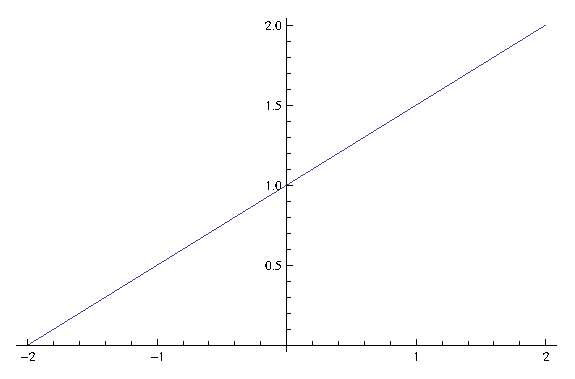
\includegraphics[width=0.45\textwidth]{continuous/functions/halfxeg}
        }
        \subfigure[A plot of $f^{-1}(x)=2x-2$.]{\
          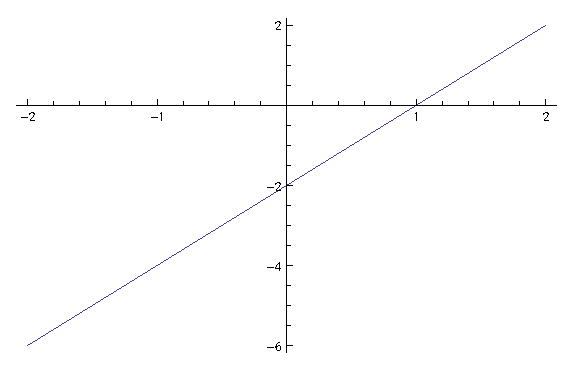
\includegraphics[width=0.45\textwidth]{continuous/functions/halfxeginv}
        }
      \end{center}
      \caption{Plots of functions from Example~\ref{ex:inverses}.}
      \label{fig:inverseg}
    \end{figure}
    Now we can test this: $f(1)=(1/2) (1) + 1=3/2$ and 
    $f^{-1}(3/2) = 2(3/2)-2 = 1$. Same for $f(0)=(1/2)(0)+1=1$;
    $f^{-1}(1) = 2(1)-2 = 0$, and for any other $x$ value we could choose.
  \end{sol}
\end{ex}
